\begin{center}
	\textbf{\Large Formation Préparatoire : Cours I}
\end{center}

\section*{Partie I : Méthodes mathématiques}

\subsection*{Équations différentielles d’ordre 1 solubles par la séparation des variables}

Trouver les solutions des équations différentielles suivantes. Pour chacune d’entre elles, trouver d’abord la solution générale et ensuite la solution particulière qui vérifie la condition initiale (ou autre) donnée.

\begin{enumerate}
	\item 
	\[
	y'(t) + 3t^2 y(t) = 0
	\quad \text{avec la condition } y(0)=2
	\]
	
	\item 
	\[
	y(t)y'(t) + t = 1
	\quad \text{avec la condition } y(0)=1
	\]
	
	\item 
	\[
	(t^3+1)y'(t) + t^2y(t)^2 = 0
	\quad \text{avec la condition } y(0)=1
	\]
\end{enumerate}

\subsection*{Équations différentielles linéaires d’ordre 1 à coefficients et second membre variables}

On se propose de résoudre l’équation différentielle du premier ordre suivante :
\[
y'(t) + 4t^3 y(t) = \exp(-t^4 + 2t)
\quad \text{avec la condition } y(0)=1
\]

Cherchez tout d’abord la solution sans second membre. Appliquez ensuite la technique de la variation de la constante pour trouver la solution particulière avec second membre et justifiant la condition aux limites.

\subsection*{Équations différentielles linéaires d’ordre 2 à coefficients et second membre variables}

On se propose de résoudre l’équation différentielle du second ordre suivante :
\[
y''(t) - 5y'(t) + 6y(t) = t\,\exp(t)
\]

\begin{enumerate}
	\item Trouver d’abord la solution générale.
	
	\item Mettez l’équation différentielle sous la forme
	\[
	\left(\frac{d}{dt}-a\right)\left(\frac{d}{dt}-b\right)y(t) = t\exp(t)
	\]
	où \(a\) et \(b\) sont deux constantes à déterminer.
	
	\item En notant
	\[
	\left(\frac{d}{dt}-b\right)y(t) = g(t),
	\]
	résoudre l’équation différentielle agissant sur \(g(t)\).
	
	\item Résoudre ensuite l’équation différentielle agissant sur \(y(t)\) qui vérifie les conditions initiales
	\[
	y(0)=0, \quad y'(0)=1.
	\]
\end{enumerate}

Observons que, au contraire des équations linéaires du premier ordre, les équations différentielles d’ordre 2 nécessitent deux conditions indépendantes (conditions initiales ou autres) pour fixer les valeurs des deux constantes d’intégration de la solution générale.

\section*{Partie II : Méthodes physiques}

\subsection*{Applications aux systèmes des équations couplées de l’oscillateur mécanique}

Le système mécanique de deux oscillateurs couplés que nous nous proposons d’étudier est présenté sur la figure 1.  
Il est composé de deux objets de masse respective \(m_1\) et \(m_2\) différentes pouvant se déplacer uniquement selon la direction horizontale, le long de l’axe \(x\).  
Dans cet état, trois ressorts de même raideur \(K\), de même longueur à l’équilibre, et attachés fixement aux deux extrémités, permettent de maintenir une force entre les deux masses.  
Nous admettons que, lors du mouvement, les ressorts sont sous tension, c’est-à-dire qu’ils ne sont pas déformés dans cet état initial.

\begin{figure}[h!]
	\centering



\tikzset{every picture/.style={line width=0.75pt}} %set default line width to 0.75pt        

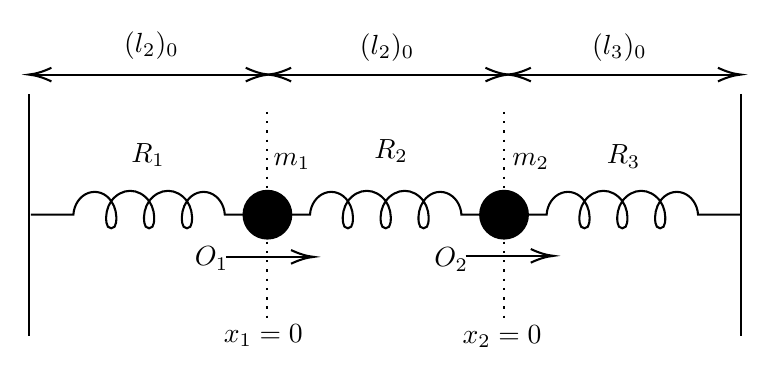
\begin{tikzpicture}[x=0.75pt,y=0.75pt,yscale=-1,xscale=1]
	%uncomment if require: \path (0,435); %set diagram left start at 0, and has height of 435
	
	%Straight Lines [id:da8139997984603213] 
	\draw    (200,108.5) -- (200,225) ;
	%Straight Lines [id:da07019762619638148] 
	\draw    (543,108.25) -- (543,224.75) ;
	%Shape: Circle [id:dp7624157630559317] 
	\draw  [fill={rgb, 255:red, 0; green, 0; blue, 0 }  ,fill opacity=1 ] (303.5,166.5) .. controls (303.5,160.15) and (308.65,155) .. (315,155) .. controls (321.35,155) and (326.5,160.15) .. (326.5,166.5) .. controls (326.5,172.85) and (321.35,178) .. (315,178) .. controls (308.65,178) and (303.5,172.85) .. (303.5,166.5) -- cycle ;
	%Shape: Circle [id:dp8917031379948387] 
	\draw  [fill={rgb, 255:red, 0; green, 0; blue, 0 }  ,fill opacity=1 ] (417.5,166.5) .. controls (417.5,160.15) and (422.65,155) .. (429,155) .. controls (435.35,155) and (440.5,160.15) .. (440.5,166.5) .. controls (440.5,172.85) and (435.35,178) .. (429,178) .. controls (422.65,178) and (417.5,172.85) .. (417.5,166.5) -- cycle ;
	%Shape: Inductor (Air Core) [id:dp1543763567402443] 
	\draw   (201,166.5) -- (221.52,166.5) .. controls (221.82,161.65) and (224.66,157.5) .. (228.69,156.05) .. controls (232.73,154.6) and (237.12,156.14) .. (239.76,159.94) .. controls (241.8,162.9) and (242.63,166.72) .. (242.04,170.44) .. controls (242.04,171.89) and (241.02,173.06) .. (239.76,173.06) .. controls (238.5,173.06) and (237.48,171.89) .. (237.48,170.44) .. controls (236.89,166.72) and (237.72,162.9) .. (239.76,159.94) .. controls (242.13,156.79) and (245.43,155) .. (248.88,155) .. controls (252.33,155) and (255.63,156.79) .. (258,159.94) .. controls (260.04,162.9) and (260.87,166.72) .. (260.28,170.44) .. controls (260.28,171.89) and (259.26,173.06) .. (258,173.06) .. controls (256.74,173.06) and (255.72,171.89) .. (255.72,170.44) .. controls (255.13,166.72) and (255.96,162.9) .. (258,159.94) .. controls (260.37,156.79) and (263.67,155) .. (267.12,155) .. controls (270.57,155) and (273.87,156.79) .. (276.24,159.94) .. controls (278.28,162.9) and (279.11,166.72) .. (278.52,170.44) .. controls (278.52,171.89) and (277.5,173.06) .. (276.24,173.06) .. controls (274.98,173.06) and (273.96,171.89) .. (273.96,170.44) .. controls (273.37,166.72) and (274.2,162.9) .. (276.24,159.94) .. controls (278.88,156.14) and (283.27,154.6) .. (287.31,156.05) .. controls (291.34,157.5) and (294.18,161.65) .. (294.48,166.5) -- (315,166.5) ;
	%Straight Lines [id:da7550159946155199] 
	\draw    (295,186.83) -- (335.33,186.83) ;
	\draw [shift={(337.33,186.83)}, rotate = 180] [color={rgb, 255:red, 0; green, 0; blue, 0 }  ][line width=0.75]    (10.93,-3.29) .. controls (6.95,-1.4) and (3.31,-0.3) .. (0,0) .. controls (3.31,0.3) and (6.95,1.4) .. (10.93,3.29)   ;
	%Straight Lines [id:da862076015559579] 
	\draw  [dash pattern={on 0.84pt off 2.51pt}]  (315,116.92) -- (315,216.08) ;
	%Shape: Inductor (Air Core) [id:dp8887708100725206] 
	\draw   (315,166.5) -- (335.52,166.5) .. controls (335.82,161.65) and (338.66,157.5) .. (342.69,156.05) .. controls (346.73,154.6) and (351.12,156.14) .. (353.76,159.94) .. controls (355.8,162.9) and (356.63,166.72) .. (356.04,170.44) .. controls (356.04,171.89) and (355.02,173.06) .. (353.76,173.06) .. controls (352.5,173.06) and (351.48,171.89) .. (351.48,170.44) .. controls (350.89,166.72) and (351.72,162.9) .. (353.76,159.94) .. controls (356.13,156.79) and (359.43,155) .. (362.88,155) .. controls (366.33,155) and (369.63,156.79) .. (372,159.94) .. controls (374.04,162.9) and (374.87,166.72) .. (374.28,170.44) .. controls (374.28,171.89) and (373.26,173.06) .. (372,173.06) .. controls (370.74,173.06) and (369.72,171.89) .. (369.72,170.44) .. controls (369.13,166.72) and (369.96,162.9) .. (372,159.94) .. controls (374.37,156.79) and (377.67,155) .. (381.12,155) .. controls (384.57,155) and (387.87,156.79) .. (390.24,159.94) .. controls (392.28,162.9) and (393.11,166.72) .. (392.52,170.44) .. controls (392.52,171.89) and (391.5,173.06) .. (390.24,173.06) .. controls (388.98,173.06) and (387.96,171.89) .. (387.96,170.44) .. controls (387.37,166.72) and (388.2,162.9) .. (390.24,159.94) .. controls (392.88,156.14) and (397.27,154.6) .. (401.31,156.05) .. controls (405.34,157.5) and (408.18,161.65) .. (408.48,166.5) -- (429,166.5) ;
	%Shape: Inductor (Air Core) [id:dp6663674815751357] 
	\draw   (429,166.5) -- (449.52,166.5) .. controls (449.82,161.65) and (452.66,157.5) .. (456.69,156.05) .. controls (460.73,154.6) and (465.12,156.14) .. (467.76,159.94) .. controls (469.8,162.9) and (470.63,166.72) .. (470.04,170.44) .. controls (470.04,171.89) and (469.02,173.06) .. (467.76,173.06) .. controls (466.5,173.06) and (465.48,171.89) .. (465.48,170.44) .. controls (464.89,166.72) and (465.72,162.9) .. (467.76,159.94) .. controls (470.13,156.79) and (473.43,155) .. (476.88,155) .. controls (480.33,155) and (483.63,156.79) .. (486,159.94) .. controls (488.04,162.9) and (488.87,166.72) .. (488.28,170.44) .. controls (488.28,171.89) and (487.26,173.06) .. (486,173.06) .. controls (484.74,173.06) and (483.72,171.89) .. (483.72,170.44) .. controls (483.13,166.72) and (483.96,162.9) .. (486,159.94) .. controls (488.37,156.79) and (491.67,155) .. (495.12,155) .. controls (498.57,155) and (501.87,156.79) .. (504.24,159.94) .. controls (506.28,162.9) and (507.11,166.72) .. (506.52,170.44) .. controls (506.52,171.89) and (505.5,173.06) .. (504.24,173.06) .. controls (502.98,173.06) and (501.96,171.89) .. (501.96,170.44) .. controls (501.37,166.72) and (502.2,162.9) .. (504.24,159.94) .. controls (506.88,156.14) and (511.27,154.6) .. (515.31,156.05) .. controls (519.34,157.5) and (522.18,161.65) .. (522.48,166.5) -- (543,166.5) ;
	%Straight Lines [id:da6017499700622293] 
	\draw  [dash pattern={on 0.84pt off 2.51pt}]  (429,116.92) -- (429,216.08) ;
	%Straight Lines [id:da11743565183506999] 
	\draw    (410.5,186.33) -- (450.83,186.33) ;
	\draw [shift={(452.83,186.33)}, rotate = 180] [color={rgb, 255:red, 0; green, 0; blue, 0 }  ][line width=0.75]    (10.93,-3.29) .. controls (6.95,-1.4) and (3.31,-0.3) .. (0,0) .. controls (3.31,0.3) and (6.95,1.4) .. (10.93,3.29)   ;
	%Straight Lines [id:da37355424967826245] 
	\draw    (202,99) -- (313.5,99) ;
	\draw [shift={(315.5,99)}, rotate = 180] [color={rgb, 255:red, 0; green, 0; blue, 0 }  ][line width=0.75]    (10.93,-3.29) .. controls (6.95,-1.4) and (3.31,-0.3) .. (0,0) .. controls (3.31,0.3) and (6.95,1.4) .. (10.93,3.29)   ;
	\draw [shift={(200,99)}, rotate = 0] [color={rgb, 255:red, 0; green, 0; blue, 0 }  ][line width=0.75]    (10.93,-3.29) .. controls (6.95,-1.4) and (3.31,-0.3) .. (0,0) .. controls (3.31,0.3) and (6.95,1.4) .. (10.93,3.29)   ;
	%Straight Lines [id:da1178951432468558] 
	\draw    (317.5,99) -- (429,99) ;
	\draw [shift={(431,99)}, rotate = 180] [color={rgb, 255:red, 0; green, 0; blue, 0 }  ][line width=0.75]    (10.93,-3.29) .. controls (6.95,-1.4) and (3.31,-0.3) .. (0,0) .. controls (3.31,0.3) and (6.95,1.4) .. (10.93,3.29)   ;
	\draw [shift={(315.5,99)}, rotate = 0] [color={rgb, 255:red, 0; green, 0; blue, 0 }  ][line width=0.75]    (10.93,-3.29) .. controls (6.95,-1.4) and (3.31,-0.3) .. (0,0) .. controls (3.31,0.3) and (6.95,1.4) .. (10.93,3.29)   ;
	%Straight Lines [id:da15086850345472147] 
	\draw    (433,99) -- (541,99) ;
	\draw [shift={(543,99)}, rotate = 180] [color={rgb, 255:red, 0; green, 0; blue, 0 }  ][line width=0.75]    (10.93,-3.29) .. controls (6.95,-1.4) and (3.31,-0.3) .. (0,0) .. controls (3.31,0.3) and (6.95,1.4) .. (10.93,3.29)   ;
	\draw [shift={(431,99)}, rotate = 0] [color={rgb, 255:red, 0; green, 0; blue, 0 }  ][line width=0.75]    (10.93,-3.29) .. controls (6.95,-1.4) and (3.31,-0.3) .. (0,0) .. controls (3.31,0.3) and (6.95,1.4) .. (10.93,3.29)   ;
	
	% Text Node
	\draw (292.5,218.07) node [anchor=north west][inner sep=0.75pt]    {$x_{1} =0$};
	% Text Node
	\draw (407.5,218.57) node [anchor=north west][inner sep=0.75pt]    {$x_{2} =0$};
	% Text Node
	\draw (278.5,180.57) node [anchor=north west][inner sep=0.75pt]    {$O_{1}$};
	% Text Node
	\draw (394,181.07) node [anchor=north west][inner sep=0.75pt]    {$O_{2}$};
	% Text Node
	\draw (248,130.9) node [anchor=north west][inner sep=0.75pt]    {$R_{1}$};
	% Text Node
	\draw (365,128.9) node [anchor=north west][inner sep=0.75pt]    {$R_{2}$};
	% Text Node
	\draw (477,131.4) node [anchor=north west][inner sep=0.75pt]    {$R_{3}$};
	% Text Node
	\draw (316.5,135.4) node [anchor=north west][inner sep=0.75pt]    {$m_{1}$};
	% Text Node
	\draw (431.5,135.4) node [anchor=north west][inner sep=0.75pt]    {$m_{2}$};
	% Text Node
	\draw (244.5,76.9) node [anchor=north west][inner sep=0.75pt]    {$( l_{2})_{0}$};
	% Text Node
	\draw (358,77.9) node [anchor=north west][inner sep=0.75pt]    {$( l_{2})_{0}$};
	% Text Node
	\draw (470,77.9) node [anchor=north west][inner sep=0.75pt]    {$( l_{3})_{0}$};
	
	
\end{tikzpicture}

	\caption{Schéma d’un oscillateur mécanique composé de deux masses de masse respective $m_1$ et $m_2$ reliées par trois ressorts de même raideur $K$.}
\end{figure}

\begin{enumerate}
	\item Comment écrivez-vous la force agissant sur chaque masse en fonction du déplacement
	de leur coordonnée respective $\delta x_1 = x_1 - x_1^0$ et $\delta x_2 = x_2 - x_2^0$
	où $x_1^0$ et $x_2^0$ représentent les positions d’équilibre respectives des deux masses ?
	
	\item Donnez l’équation du mouvement mécanique pour les deux masses en fonction de
	$m_1$, $m_2$ et $K$ avec $m_2 \neq m_1$.  
	Quelle est l’unité du rapport des grandeurs $K/m_{1,2}$ ?
	À quelle grandeur physique correspond ce rapport ?
	
	\item Mettre ces deux équations sous une forme matricielle en fonction des deux
	coordonnées (vecteurs déplacements) $\delta x_1$ et $\delta x_2$ écrites sous la forme
	d’un vecteur colonne.
	
	\item Comment résout-on une telle équation couplée en dehors de la solution triviale
	$\delta x_1 = \delta x_2 = 0$ correspondant à la position d’équilibre ?
	Qu’appelle-t-on modes propres (\emph{eigenmodes}) ?
	Combien de modes propres existe-t-il ? Commentez.
	
	\item Donnez les caractéristiques des modes propres : pulsations propres dans le cas
	général où $m_2 \neq m_1$, ainsi que les vecteurs propres dans le cas particulier de
	masses identiques ($m_2 = m_1$).
	
	\item Les masses sont désormais identiques. À l’instant $t=0$, on écarte la masse 1 de sa
	position d’équilibre d’une valeur $\delta x_1(t=0) = \Delta$.  
	Donnez l’équation de mouvement des deux masses couplées.
\end{enumerate}



